\documentclass{article}
\usepackage{tikz,pgfplots}
\usepackage{tikz-qtree}
\usepackage{units}
\pgfplotsset{compat=1.8}
%\pgfplotsset{colormap={mix}{
%	color(0cm)=(blue);
%	color(1cm)=(green);
%	color(2cm)=(yellow)
%	color(3cm)=(red)}}

\usetikzlibrary{patterns,shadows,trees,calc}

\definecolor{diplom1}{rgb}{0.0 0.4 1.0}
\definecolor{diplom2}{rgb}{0.0 0.0 0.6}
\definecolor{diplom3}{RGB}{153,0,0} %unirot
\definecolor{diplom4}{RGB}{232,215,23}
\definecolor{diplom5}{RGB}{51,37,60}

\definecolor{unirot}{RGB}{153,0,0}
\definecolor{unirot_hell}{RGB}{255,228,225}
\definecolor{lightblue}{RGB}{242.2,249.88,255}

\pgfplotsset{colormap={diplom1s}{
       color(0cm)=(white);
       color(1cm)=(diplom1);
       color(10cm)=(diplom1)}}
\pgfplotsset{colormap={diplom2s}{
       color(0cm)=(white);
       color(1cm)=(diplom1);
       color(2cm)=(diplom2)}}
\pgfplotsset{colormap={blues}{
       color(0cm)=(diplom2);
       color(1cm)=(diplom1);
       color(2cm)=(white);
       color(3cm)=(diplom1);
       color(4cm)=(diplom2)}}


\begin{document}

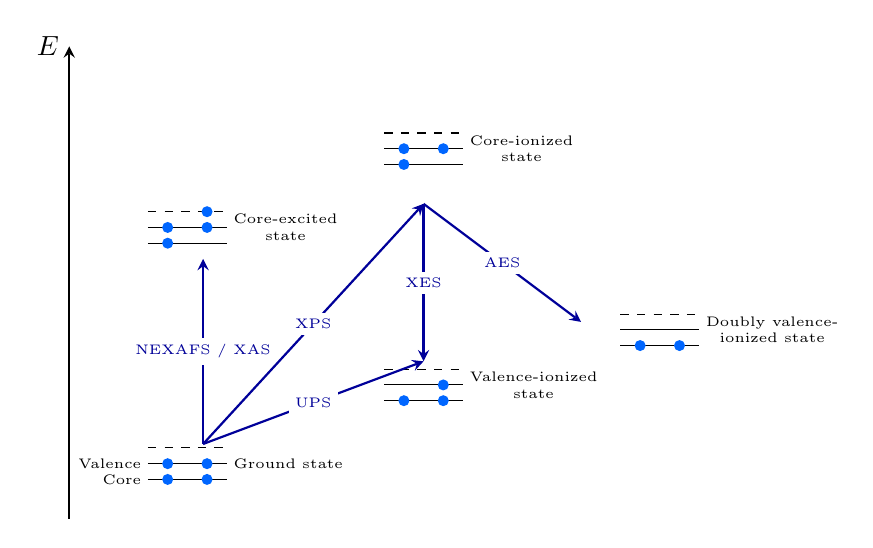
\begin{tikzpicture}[
          scale=1.0,>=stealth
        ]
%     \tiny
 % \draw[very thin,color=gray] (-0.1,-4.1) grid (10.9,4.9);
 \draw [->, thick] (0,0) -- (0,6) node [left]{$E$};
 \tiny
 \draw (1,0.5) node[left]{Core}  -- (2,0.5);
 \fill [diplom1] (1.25,0.5) circle (0.07);
 \fill [diplom1] (1.75,0.5) circle (0.07);
 \draw (1,0.7) node[left]{Valence} -- (2,0.7) node[right]{Ground state};
 \fill [diplom1] (1.25,0.7) circle (0.07);
 \fill [diplom1] (1.75,0.7) circle (0.07);
 \draw[dashed] (1,0.9) -- (2,0.9);

\begin{scope}[yshift=3cm]
 \draw (1,0.5) -- (2,0.5);
 \fill [diplom1] (1.25,0.5) circle (0.07);
 \draw (1,0.7)  -- (2,0.7) node[right, align=center]{Core-excited\\state};
 \fill [diplom1] (1.25,0.7) circle (0.07);
 \fill [diplom1] (1.75,0.7) circle (0.07);
 \draw[dashed] (1,0.9) -- (2,0.9);
 \fill [diplom1] (1.75,0.9) circle (0.07);
\end{scope}

\begin{scope}[xshift=3cm,yshift=4cm]
 \draw (1,0.5) -- (2,0.5);
 \fill [diplom1] (1.25,0.5) circle (0.07);
 \draw (1,0.7)  -- (2,0.7) node[right, align=center]{Core-ionized\\state};
 \fill [diplom1] (1.25,0.7) circle (0.07);
 \fill [diplom1] (1.75,0.7) circle (0.07);
 \draw[dashed] (1,0.9) -- (2,0.9);
\end{scope}

\begin{scope}[xshift=3cm,yshift=1cm]
 \draw (1,0.5) -- (2,0.5);
 \fill [diplom1] (1.25,0.5) circle (0.07);
 \fill [diplom1] (1.75,0.5) circle (0.07);
 \draw (1,0.7)  -- (2,0.7) node[right, align=center]{Valence-ionized\\state};
 \fill [diplom1] (1.75,0.7) circle (0.07);
 \draw[dashed] (1,0.9) -- (2,0.9);
\end{scope}

\begin{scope}[xshift=6cm,yshift=1.7cm]
 \draw (1,0.5) -- (2,0.5);
 \fill [diplom1] (1.25,0.5) circle (0.07);
 \fill [diplom1] (1.75,0.5) circle (0.07);
 \draw (1,0.7)  -- (2,0.7) node[right, align=center]{Doubly valence-\\ionized state};
 \draw[dashed] (1,0.9) -- (2,0.9);
\end{scope}

\coordinate (GS) at (1.7,0.95);
\coordinate (CES) at (1.7,3.30);
\coordinate (CIS) at (4.5,4.00);
\coordinate (VIS) at (4.5,2.00);
\coordinate (DVIS) at (6.5,2.50);

\draw [thick,diplom2,->] (GS) -- (CES);
\node [fill=white] at ($ (GS)!0.5!(CES) $) {\color{diplom2}NEXAFS / XAS};

\draw [thick,diplom2,->] (GS) -- (CIS);
\node [fill=white] at ($ (GS)!0.5!(CIS) $) {\color{diplom2}XPS};
 
\draw [thick,diplom2,->] (GS) -- (VIS);
\node [fill=white] at ($ (GS)!0.5!(VIS) $) {\color{diplom2}UPS};
 
\draw [thick,diplom2,->] (CIS) -- (VIS);
\node [fill=white] at ($ (CIS)!0.5!(VIS) $) {\color{diplom2}XES};
 
\draw [thick,diplom2,->] (CIS) -- (DVIS);
\node [fill=white] at ($ (CIS)!0.5!(DVIS) $) {\color{diplom2}AES};
 
\end{tikzpicture}

\end{document}
